\documentclass[12pt,a4paper,hidelinks]{article}


\usepackage[space]{grffile}
\usepackage[utf8]{inputenc}
\usepackage{bookmark}
\usepackage{fancyhdr}
\usepackage{libertine}
\usepackage[font=scriptsize,labelfont=bf]{caption}
\usepackage{hyperref}
\usepackage{graphicx}
\usepackage{caption}
\usepackage{times}
\usepackage{amsmath}
\usepackage{accents}
\usepackage{verbatim}
\usepackage{silence,lmodern}
\usepackage{geometry}
\usepackage{algorithm}
\usepackage{algorithmicx}
\usepackage[noend]{algpseudocode}
\usepackage[section]{placeins}

\setlength\parindent{0pt}

\captionsetup[figure]{position=above}

\hypersetup{colorlinks=false}

\geometry{
  a4paper,
  total={150mm,237mm},
  left=30mm,
  top=30mm,
}

\fancyhf{}
\rfoot{\thepage}
\pagestyle{fancy}

\floatname{algorithm}{Pseudocódigo}
\renewcommand{\figurename}{Figura}
\renewcommand\refname{}

\renewcommand{\headrulewidth}{0pt}
\renewcommand{\footrulewidth}{0.7pt}

\renewcommand\thesection{\arabic{section}.}
\renewcommand\thesubsection{\thesection\arabic{subsection}.}
\renewcommand\thesubsubsection{\thesubsection\arabic{subsubsection}.}
\renewcommand{\theequation}{\thesection\arabic{equation}}
\renewcommand{\thefigure}{\thesection\arabic{figure}}

\algrenewcommand\algorithmicrequire{\textbf{Pré-condição:}}
\algrenewcommand\algorithmicensure{\textbf{Pós-condição:}}

\newcommand*\Let[2]{\State #1 $\gets$ #2}

\captionsetup[figure]{font=normalsize}


\begin{document}

  
\hypersetup{pageanchor=false}

\begin{titlepage}
  \begin{center}
    {\large
    \textbf{Centro Federal de Educação Tecnológica de Minas Gerais}
    }

    \vspace{0.5cm}

    {\normalsize
    \textbf{Programa de Pós Graduação em Modelagem Matemática Computacional}
    }

    \vspace{2.5cm}

    {\LARGE \textbf{Caminhada Aleatória}} \\
    \vspace{0.5cm}
    {\Large \textbf{Distribuições Uniforme, Gaussiana e q-Gaussiana}}

    \vspace{3.5cm}
  \end{center}

  Breno Martins da Costa Corrêa e Souza
  (\href{mailto:breno.ec@gmail.com}{breno.ec@gmail.com}) \\
  \indent \textbf{Na condição de aluno regular de mestrado}

  \vspace{1cm}

  Allbens Atman Picardi Faria
  (\href{mailto:atman@dppg.cefetmg.br}{atman@dppg.cefetmg.br}) \\
  \indent \textbf{Professor}

  \vspace{1cm}

  \begin{center}
    \textbf{Disciplina} \\
    Modelagem de Sistemas Complexos \\
    Segundas e Quartas-feiras, 10:40 às 12:20 \\

    \vspace{1cm}

    Av.  Amazonas, 7675 - Nova Gameleira, Belo Horizonte - MG, 30510-000 \\
    Prédio 07 \\

    \vspace{3.5cm}

    \rule[1pt]{360pt}{1pt} \\

    \vspace{0.5cm}

    Belo Horizonte, 2016

  \end{center}

  \pagebreak
\end{titlepage}

\hypersetup{pageanchor=true}


  
\section{Objetivo}

O objetivo é simular caminhadas aleatórias para as seguintes distribuições:

\begin{itemize}
  \item Uniforme
  \item Gaussian
  \item q-Gaussiana, $q \in \{ 0.5, 1.5, 2.0, 2.5 \}$
\end{itemize}

  
\section{Introdução}

A Caminhada Aleatória é uma abstração de um fenômeno físico, simulada em
sistemas computacionais, que possui similaridade no eixo $x$.

\vspace{5mm}
Se construírmos gráficos de caminhadas aleatorias distintas sobre um mesmo
sistema de eixos, poderemos observar a fomação de um envelope, limitado por
valor proporcional a $t^{1/2}$. A raiz da média quadrádica dos pontos gerados
para diferentes caminhadas em determinado passo $t$ se aproximará do limite do
envelope, à medida que aumentarmos o número de caminhadas.

\vspace{5mm}
O expoente do envelope é o expoente de difusão, que é um dos expoentes que
caracterizam a classe de universalidade na qual a Caminhada Aleatória está
inserida.

  
\section{Materiais e Métodos}

As simulações tem teor probabilístico. Logo, se mostrou necessária a
implementação de um gerador de números pseudoaleatórios; portanto. O gerador
implementado foi o \texttt{Ranq2} \cite{Press:Numerical:Recipes}.

\vspace{5mm}
O método generalizado de box-müller \cite{Tsallis:2007:GeneralizedBoxMuller}
foi utilizado para gerar as distribuições Gaussiana e q-Gaussiana. O método
utiliza dois valores pseudoaleatórios gerados uniformemente para gerar um par
de valores na distribuição desejada.

\vspace{5mm}
O Pseudocódigo \ref{alg:rand-gaussian} mostra o procedimento para a geração
de um par através do método, para distribuição Gaussiana. É necessário
substituir a função logaritmo pela função q-logaritmo de $q\prime$ para
gerarmos um par na distribuição q-Gaussiana:

\begin{equation}
  q \in (-\infty, 3), \quad q \neq 1,
\end{equation}

\begin{equation}
  q\prime = \frac{1+q}{3-q},
\end{equation}

\begin{equation}
  x > 0,
\end{equation}

\begin{equation}
  ln_q = \frac{x^{1-q}-1}{1-q}.
\end{equation}

\begin{algorithm}
  \caption{Gerador de números pseudoaleatórios para Gaussiana}
  \label{alg:rand-gaussian}

  \begin{algorithmic}[1]
    \Function{RandomGaussian}{}
    \Statex

      \Let{$n_1$}{\texttt{Ranq2}} \Comment{$n \in [0,1)$}
      \Let{$n_2$}{\texttt{Ranq2}}
      \Statex

      \Let{$z_1$}{$\sqrt{\smash[b]{-2 \:ln(n_1)}} \:\cos(2 \:\pi \:u_2)$}
      \Let{$z_2$}{$\sqrt{\smash[b]{-2 \:ln(n_1)}} \:\sin(2 \:\pi \:u_2)$}
      \Statex
    \EndFunction
  \end{algorithmic}
\end{algorithm}

\vspace{5mm}
Para todas as distribuições, o passo do caminhante é o valor gerado pelo gerador
de números pseudoaleatório.

\vspace{5mm}
Cada simulação gera 2 grupos de 10 caminhadas aleatórias, com 10.000 passos,
para cada distribuição. Cada elemento do par gera um grupo distinto de
caminhadas.

  % 
\section{Discussão dos Resultados}

  
\section{Resultados}

Para cada distribuição, são apresentadas as simulações de pares ($n_1, n_2$ e
$z_1, z_2$ são pares) para escala normal e logarítmica. Curvas de
$n_1$ e $z_1$ à esquerda; $n_2$ e $z_2$ à direita.

\vspace{5mm}
O eixo $x$ representa o tempo, enquanto que o eixo $y$ representa distância
caminhada em relação à origem (0). O sistema tem dimensão $1+1$.

\vspace{5mm}
A curva de cor preta em destaque é a curva correspondente a $f(t) = t^{1/2}$. A
curva cinza em destaque é a curva correspondente à raiz da média quadrádica dos
pontos das curvas em determinado instante $t$.

  
\section{Conclusões}

A raiz da média quadrática para o caminhante q-Gaussiano, com valor $q > 5/3$,
parece violar o envelope do caminhante aleatório, caracterizado por
$f(t) = t^{1/2}$.

\vspace{5mm}
Para que possamos estimar o expoente de difusão e validá-lo com a estimativa
presente na literatura, se mostrou necessário simular um maior número de
caminhadas. Isso se dá pelo fato de que há um número considerável de saltos
abruptos na curva da raiz da média quadrática, que dificulta o ajuste.

\vspace{5mm}
Caso o expoente de difusão seja superior a $1/2$, a Caminhada Aleatória com
passo q-Gaussiano poderá simular comportamentos superdifusivos, que se enquadra
como difusão anômala.


  \begin{figure}[htb]
    \caption{Distribuição uniforme}
    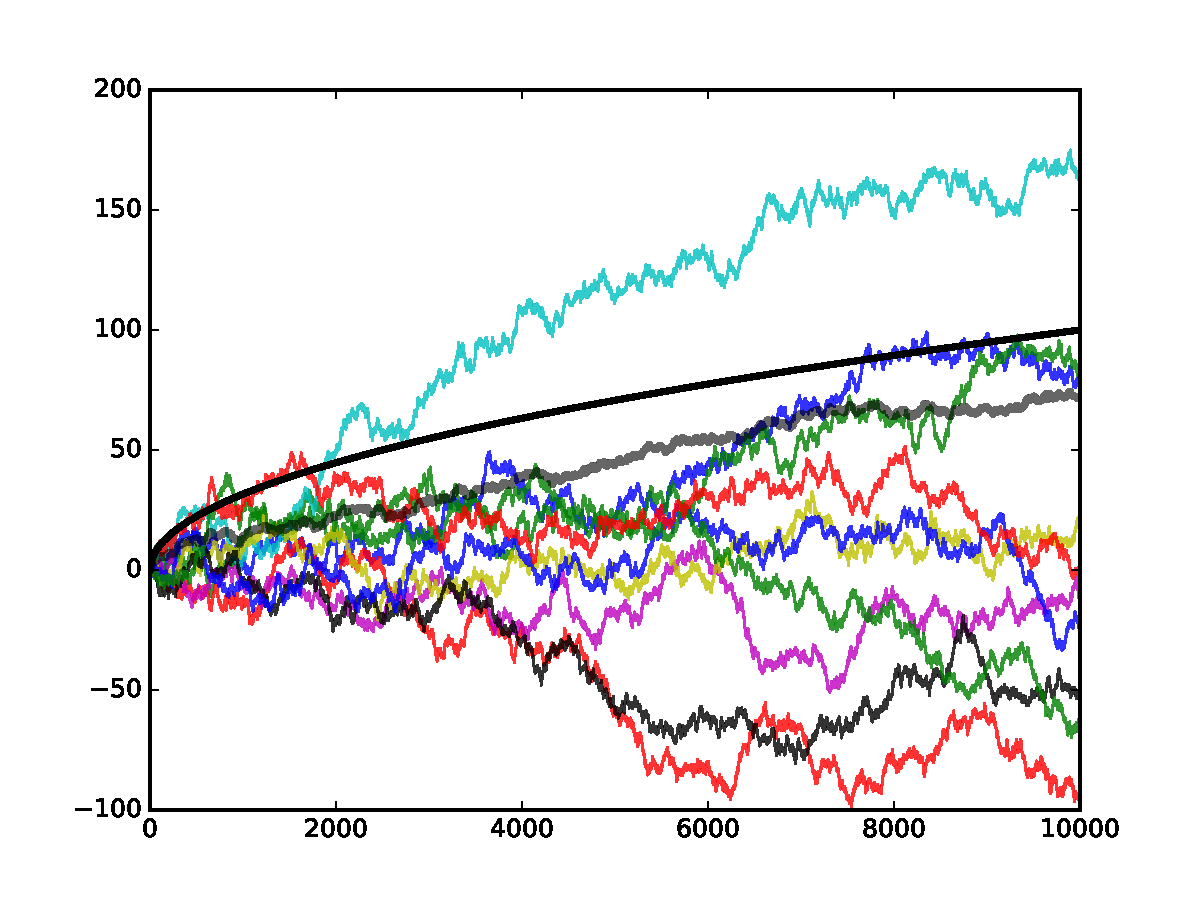
\includegraphics[width=0.5\textwidth]{figures/uni__0.pdf}
    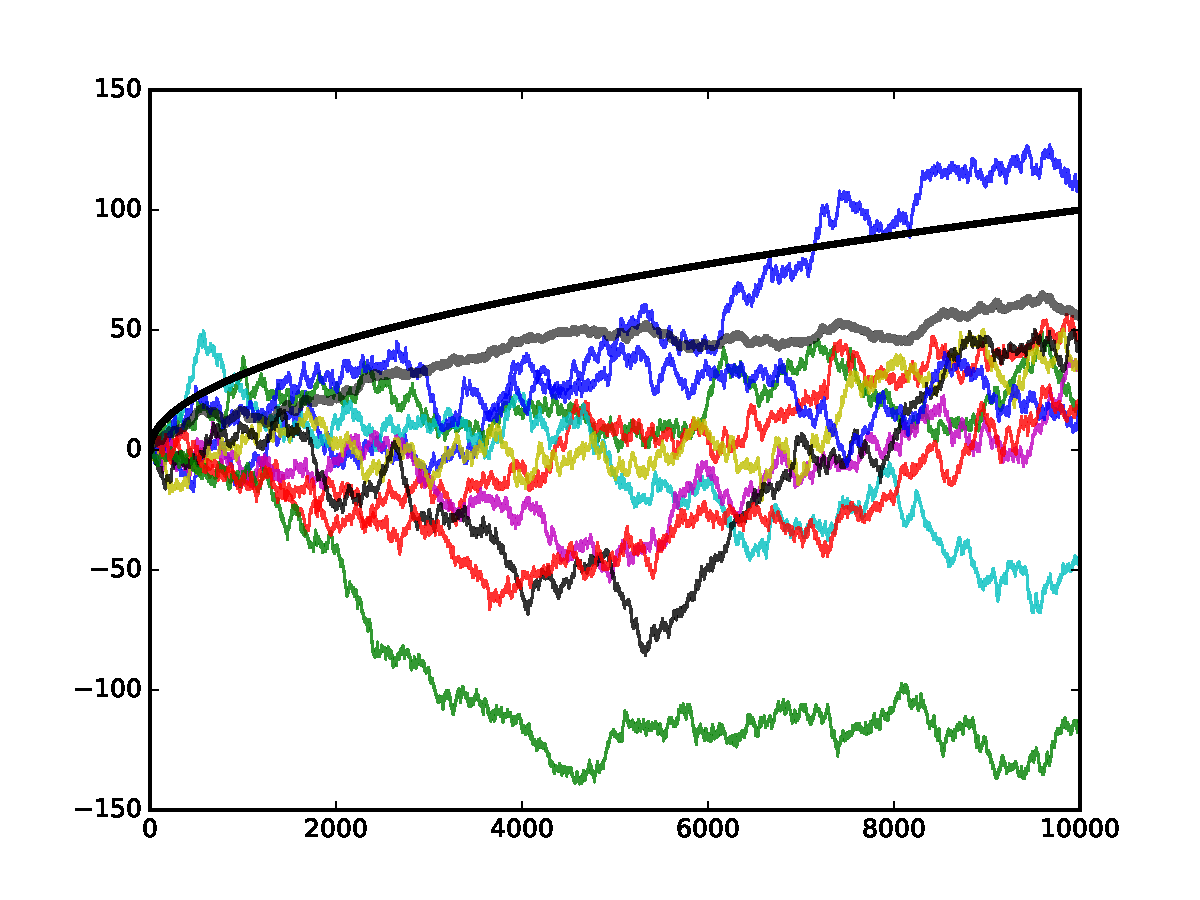
\includegraphics[width=0.5\textwidth]{figures/uni__1.pdf}
    \label{fig:randomwalk_uniform}
  \end{figure}

  \begin{figure}[htb]
    \caption{Distribuição uniforme (escala log)}
    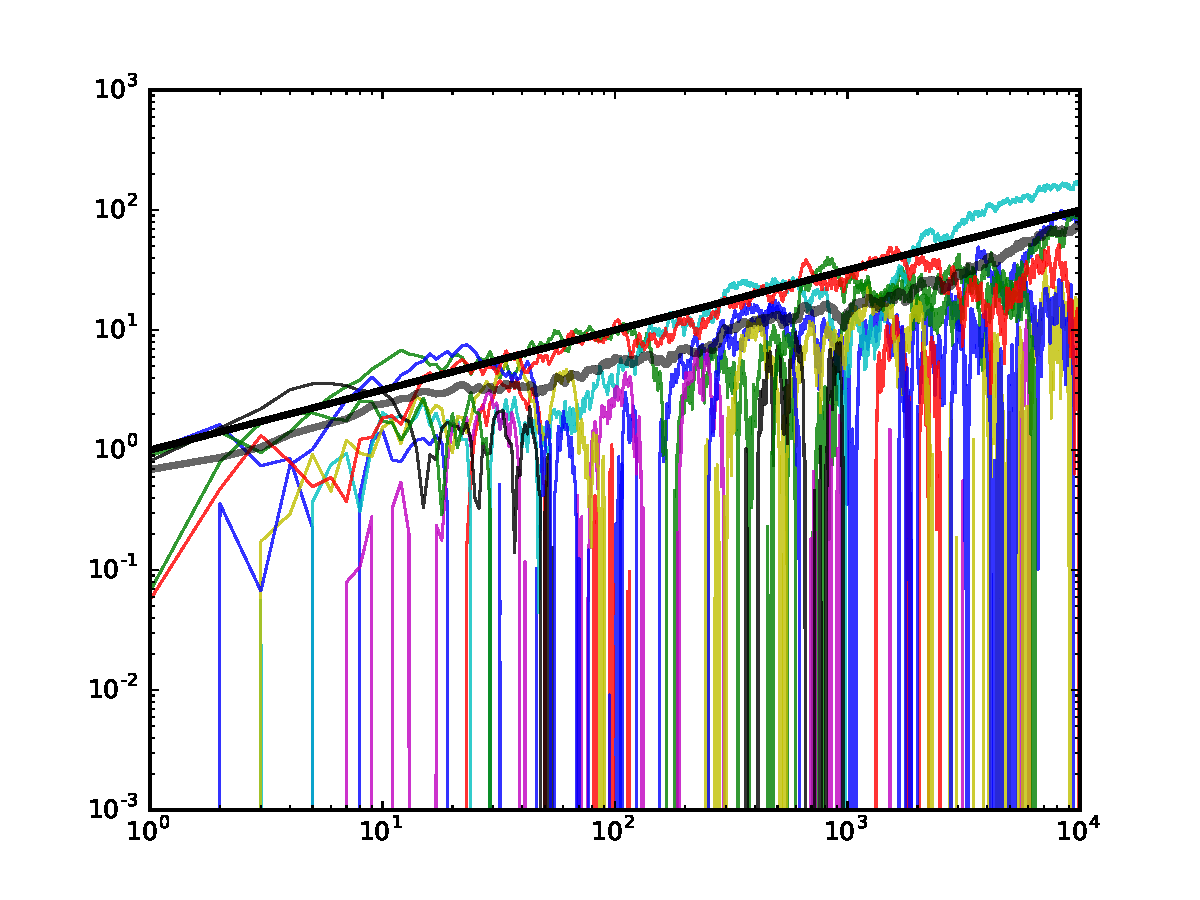
\includegraphics[width=0.5\textwidth]{figures/uni__0__log.pdf}
    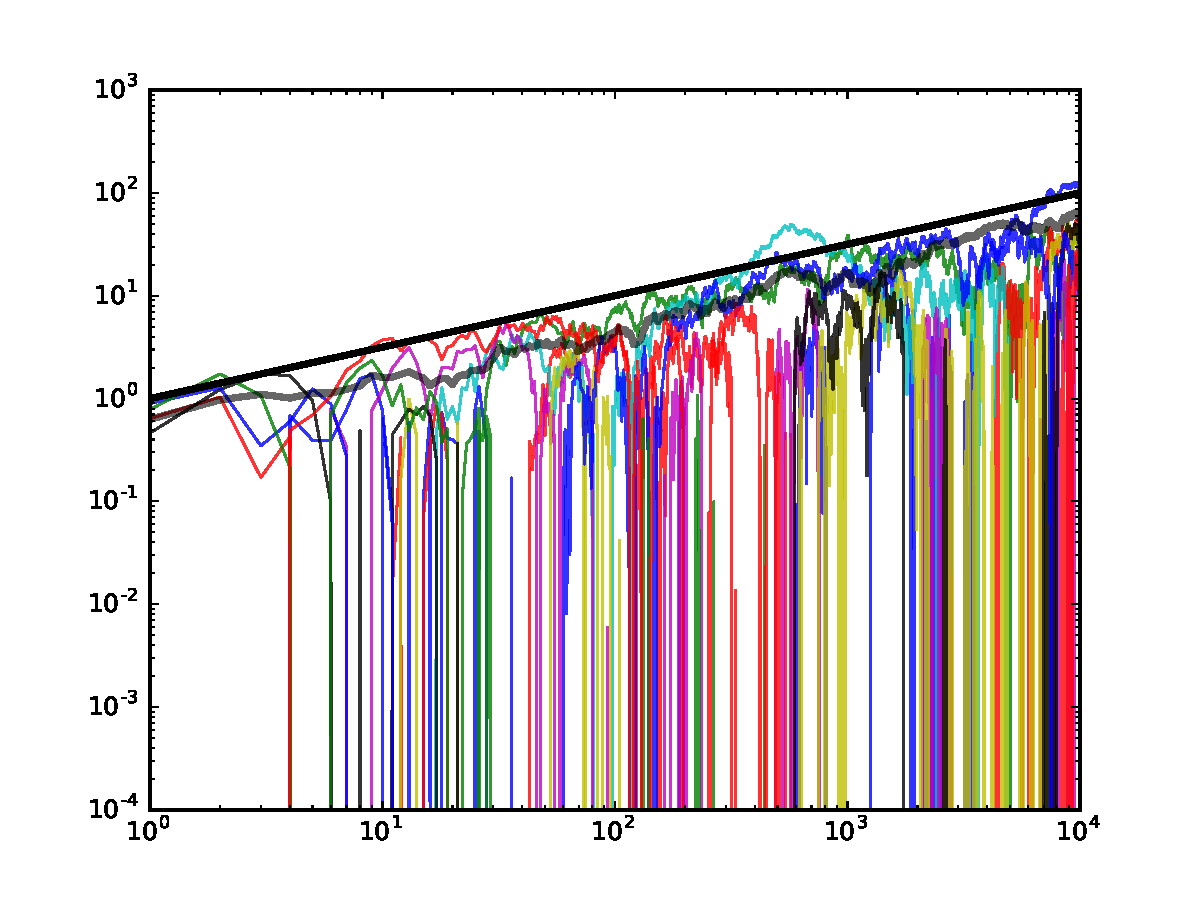
\includegraphics[width=0.5\textwidth]{figures/uni__1__log.pdf}
    \label{fig:randomwalk_uniform_log}
  \end{figure}

  \pagebreak

  \begin{figure}[htb]
    \caption{Distribuição q-Gaussiana ($q = 0.5$)}
    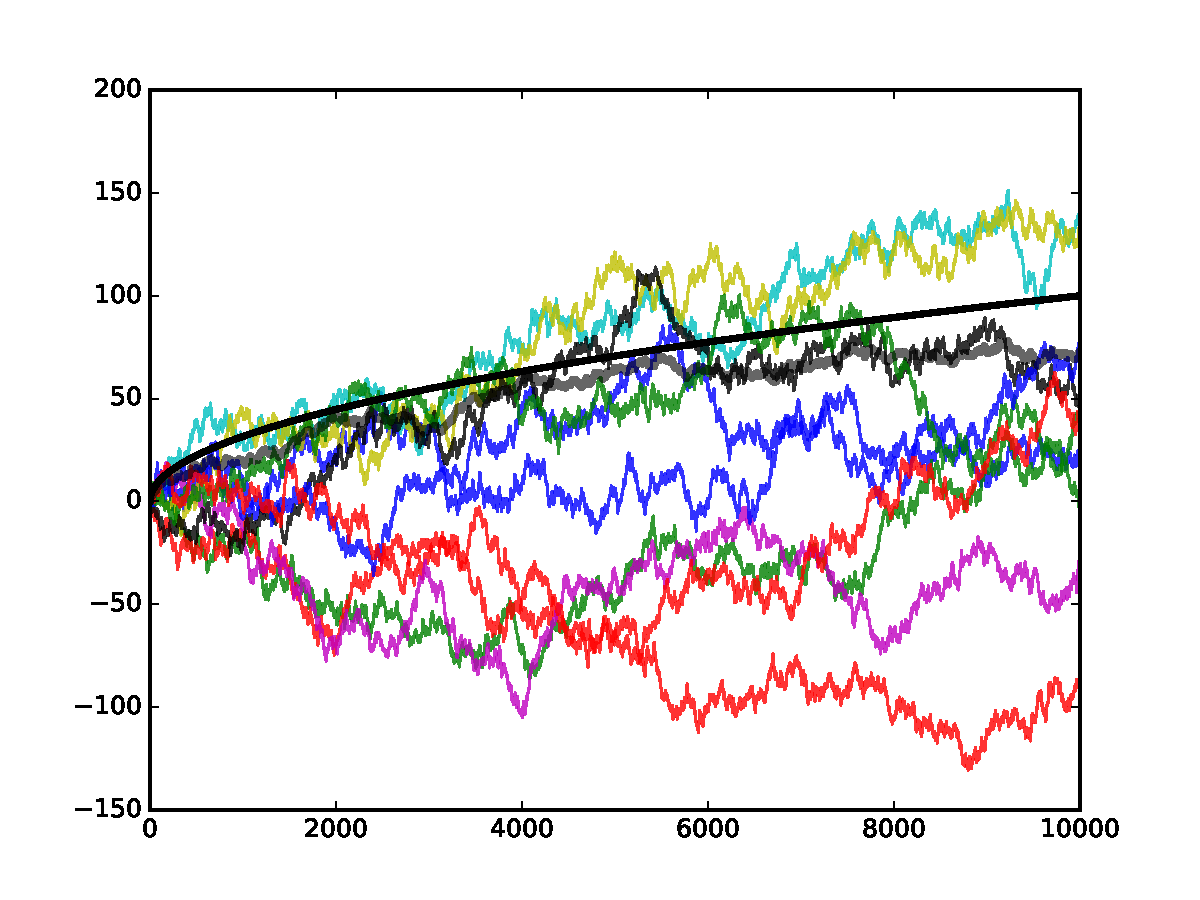
\includegraphics[width=0.5\textwidth]{figures/0_5__0.pdf}
    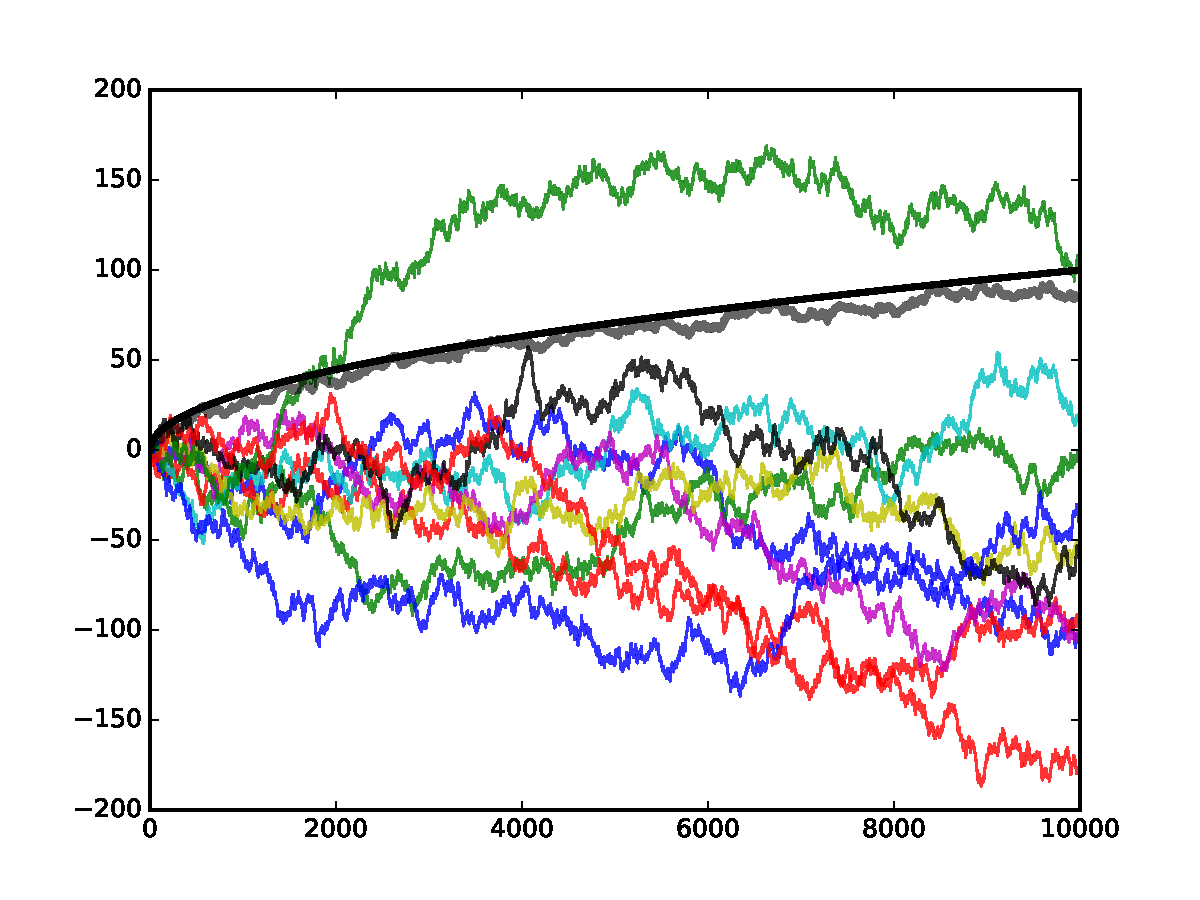
\includegraphics[width=0.5\textwidth]{figures/0_5__1.pdf}
    \label{fig:randomwalk_q-gaussian_0.5}
  \end{figure}

  \begin{figure}[htb]
    \caption{Distribuição q-Gaussiana ($q = 0.5$, escala log)}
    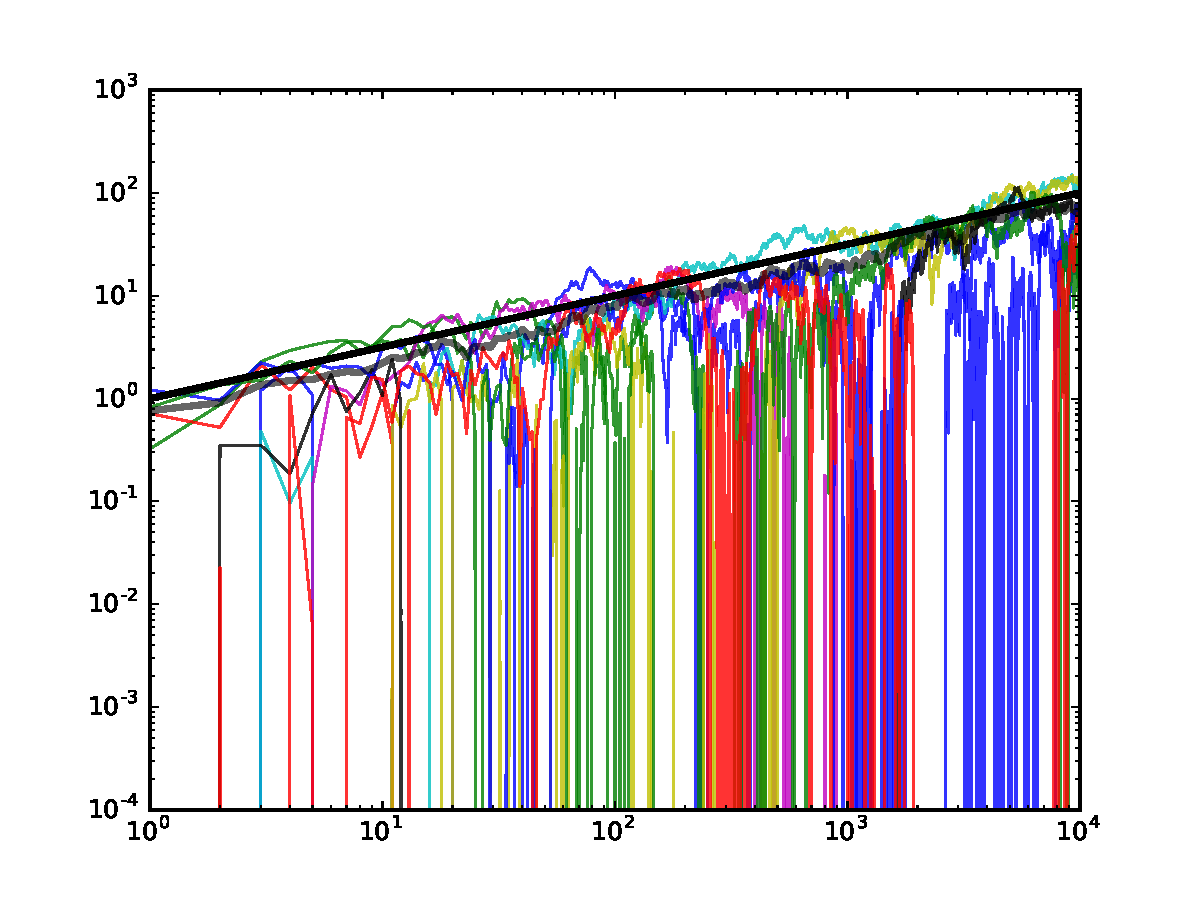
\includegraphics[width=0.5\textwidth]{figures/0_5__0__log.pdf}
    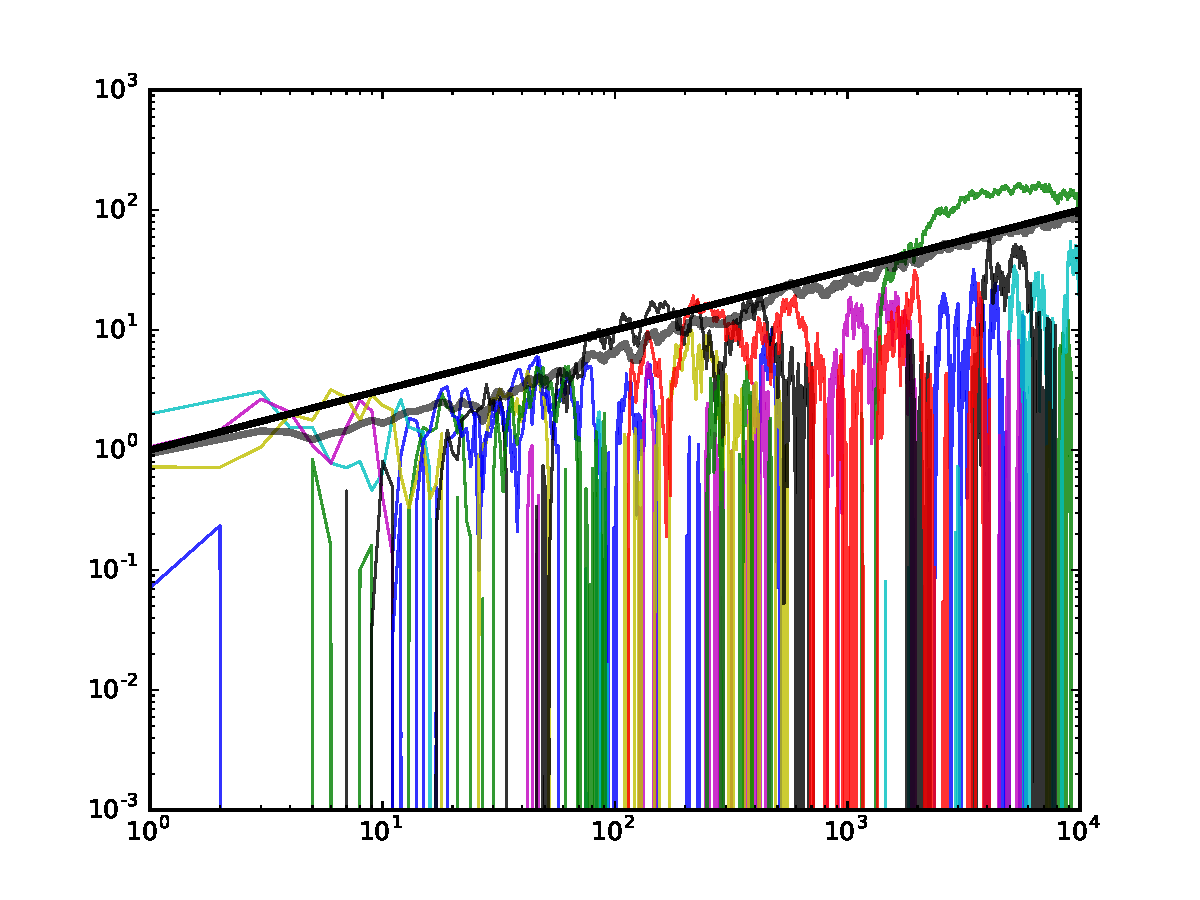
\includegraphics[width=0.5\textwidth]{figures/0_5__1__log.pdf}
    \label{fig:randomwalk_q-gaussian_0.5_log}
  \end{figure}

  \pagebreak

  \begin{figure}[htb]
    \caption{Distribuição Gaussiana ($q = 1.0$)}
    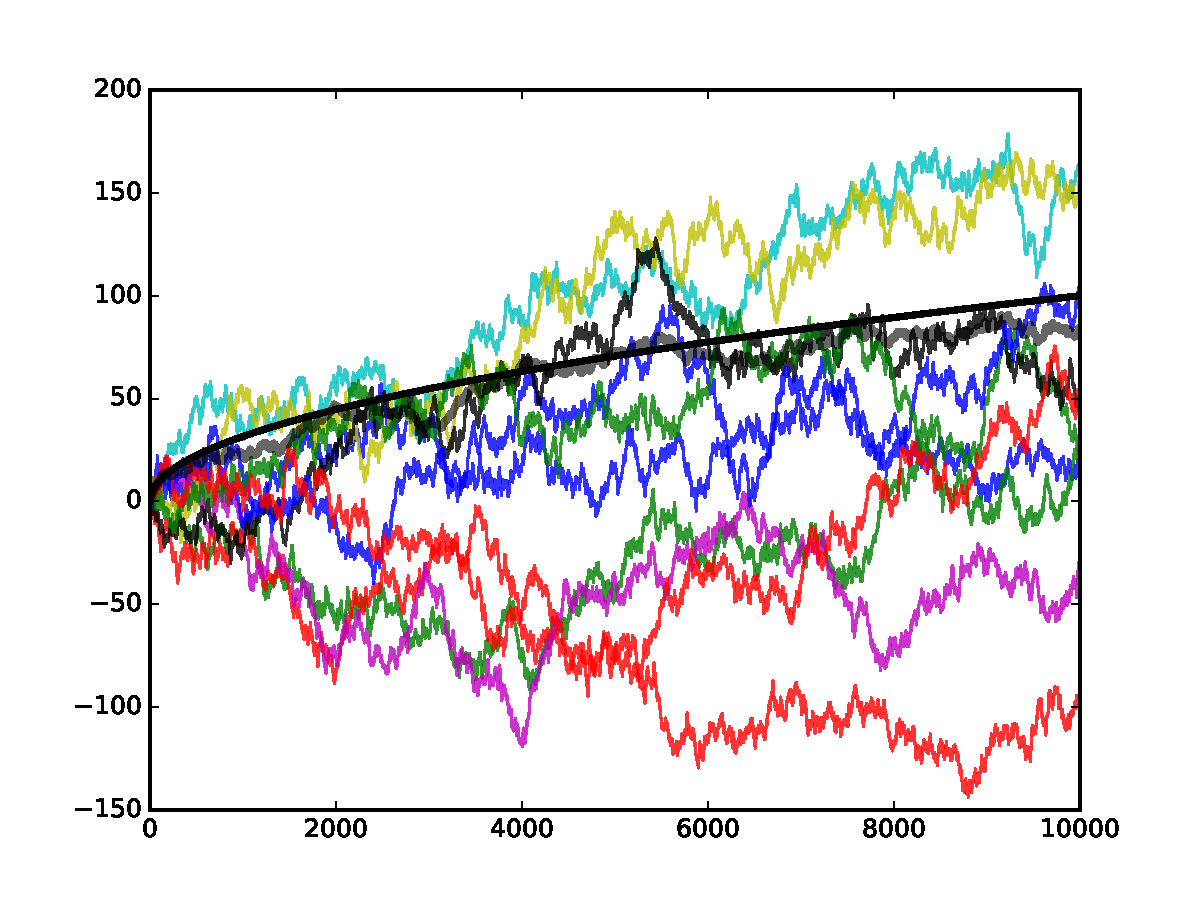
\includegraphics[width=0.5\textwidth]{figures/1_0__0.pdf}
    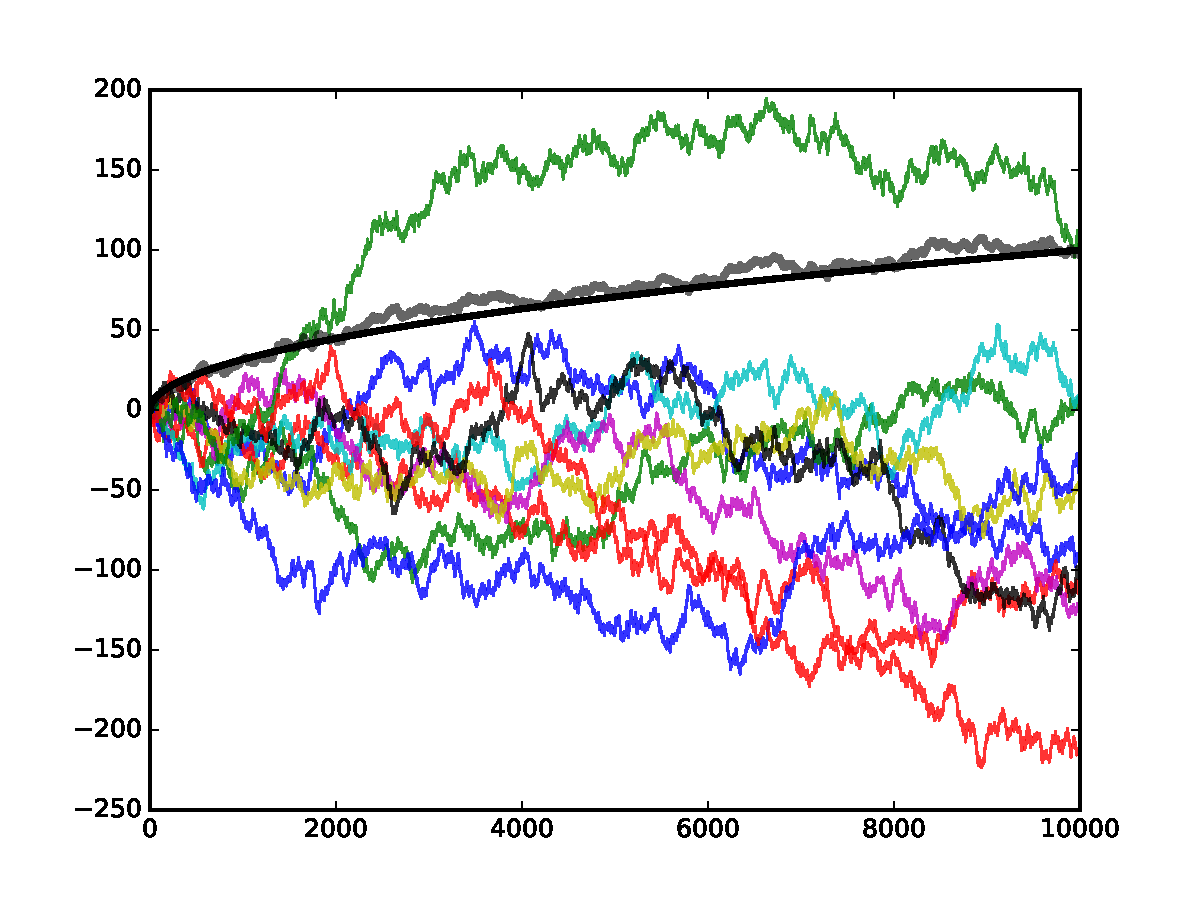
\includegraphics[width=0.5\textwidth]{figures/1_0__1.pdf}
    \label{fig:randomwalk_gaussian}
  \end{figure}

  \begin{figure}[htb]
    \caption{Distribuição Gaussiana ($q = 1.0$, escala log)}
    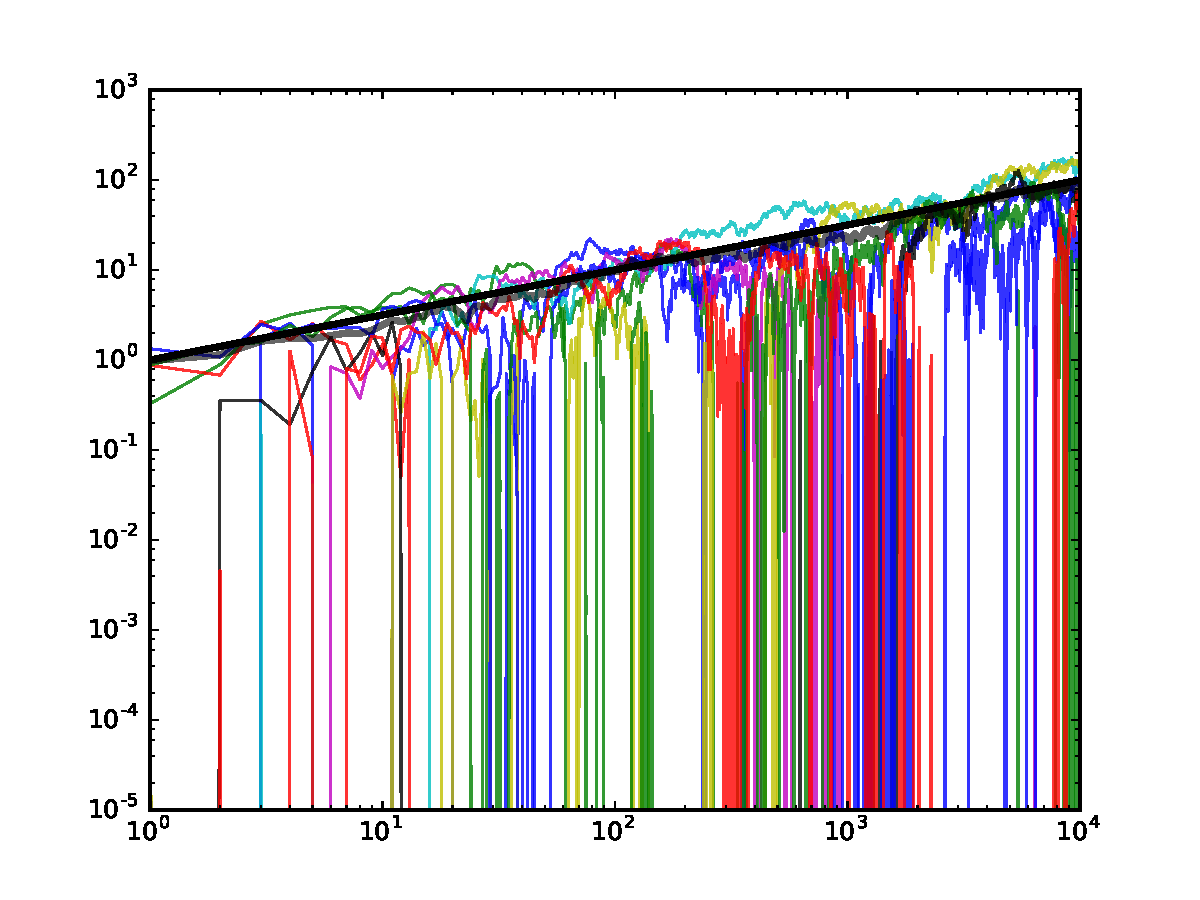
\includegraphics[width=0.5\textwidth]{figures/1_0__0__log.pdf}
    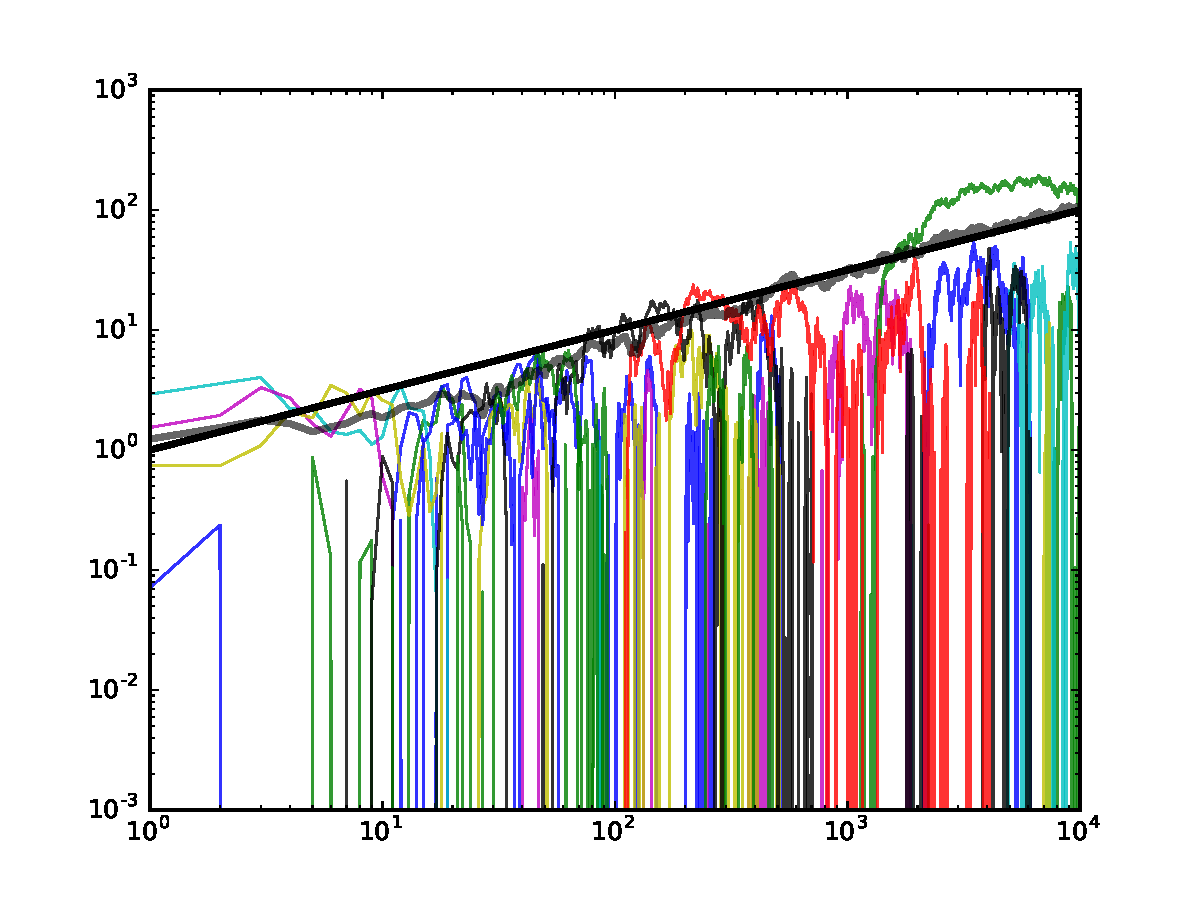
\includegraphics[width=0.5\textwidth]{figures/1_0__1__log.pdf}
    \label{fig:randomwalk_gaussian_log}
  \end{figure}

  \pagebreak

  \begin{figure}[htb]
    \caption{Distribuição q-Gaussiana ($q = 1.5$)}
    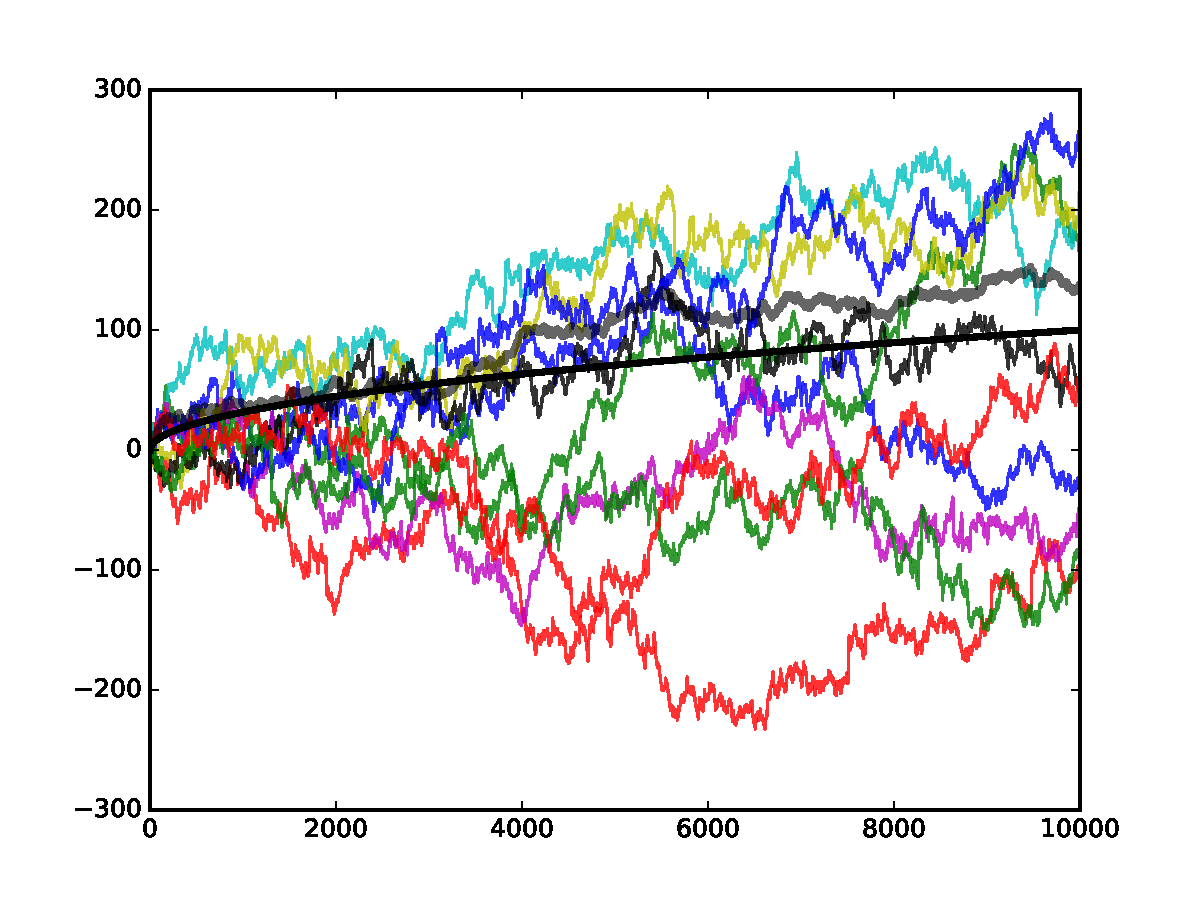
\includegraphics[width=0.5\textwidth]{figures/1_5__0.pdf}
    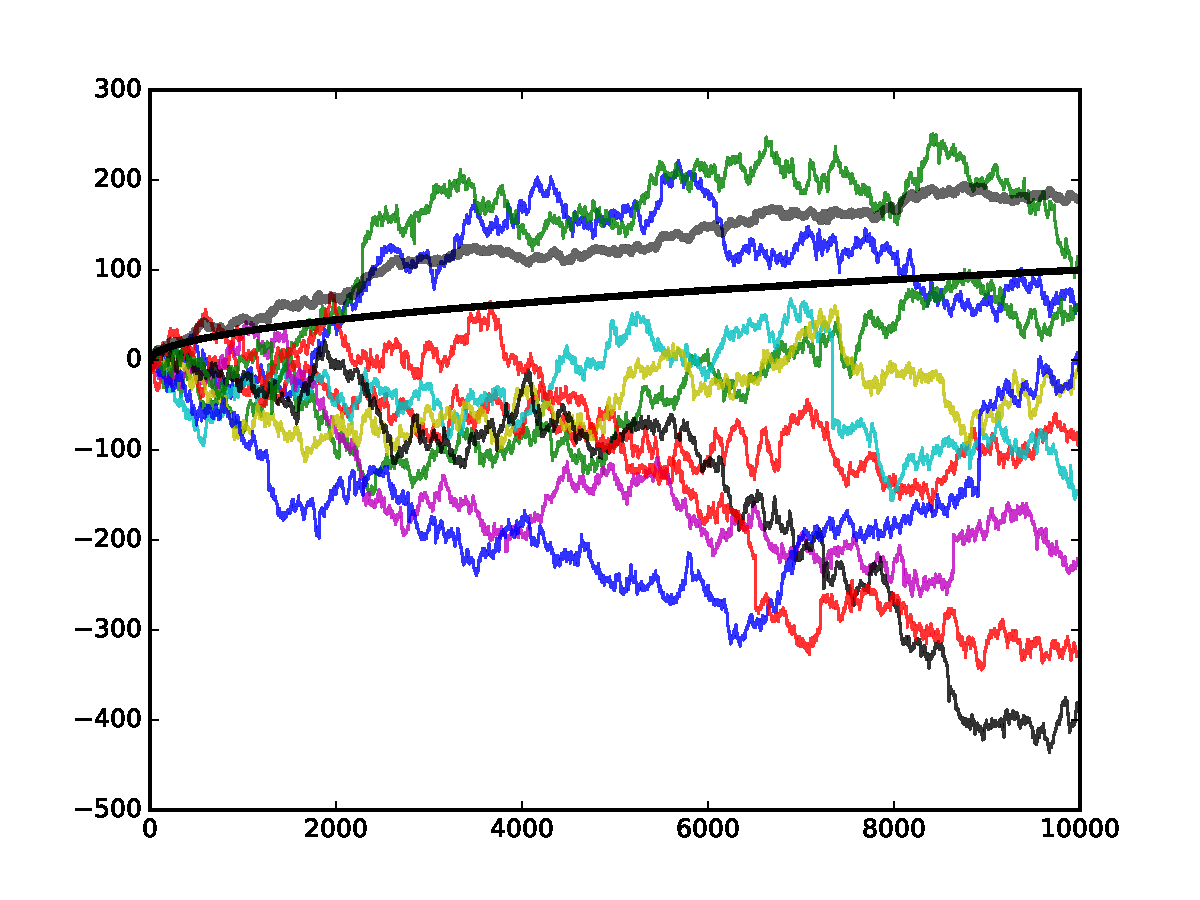
\includegraphics[width=0.5\textwidth]{figures/1_5__1.pdf}
    \label{fig:randomwalk_q-gaussian_1.5}
  \end{figure}

  \begin{figure}[htb]
    \caption{Distribuição q-Gaussiana ($q = 1.5$, escala log)}
    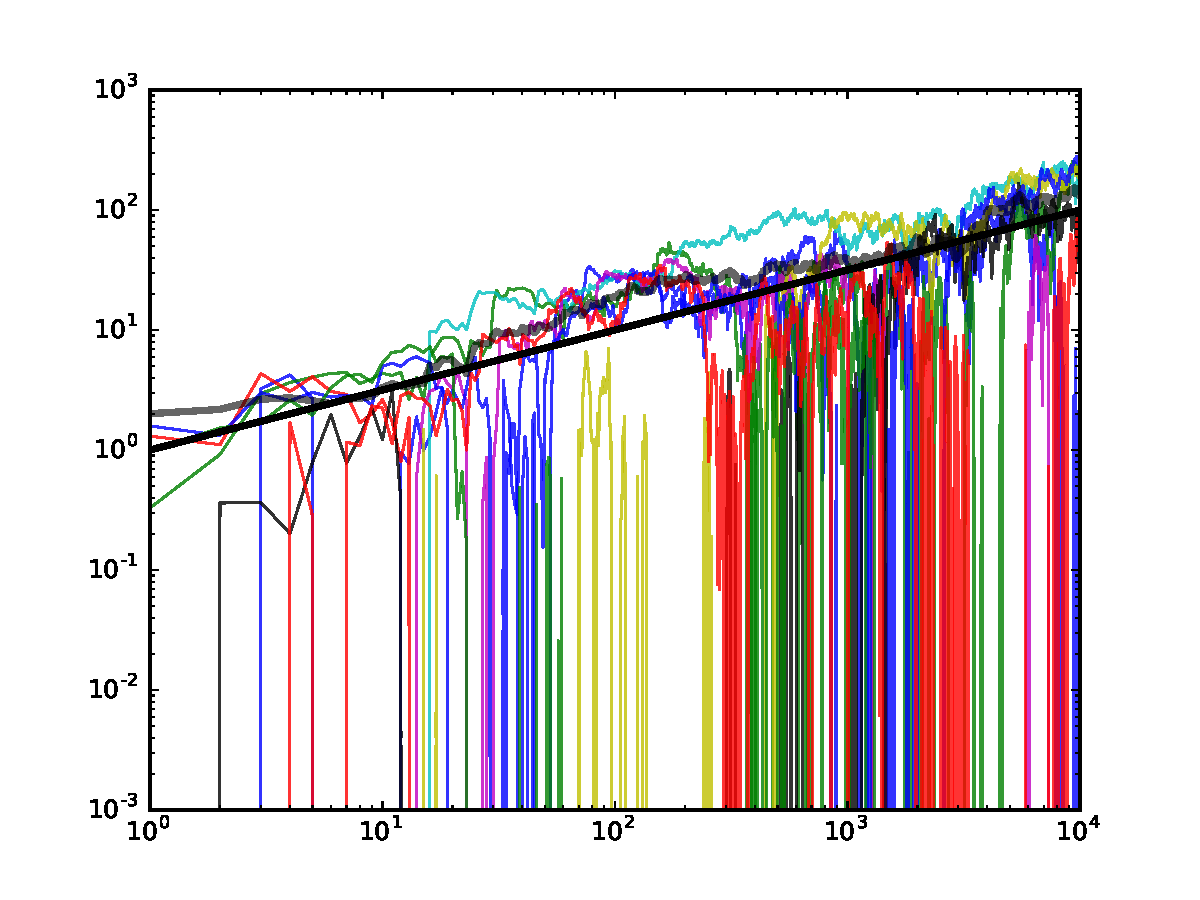
\includegraphics[width=0.5\textwidth]{figures/1_5__0__log.pdf}
    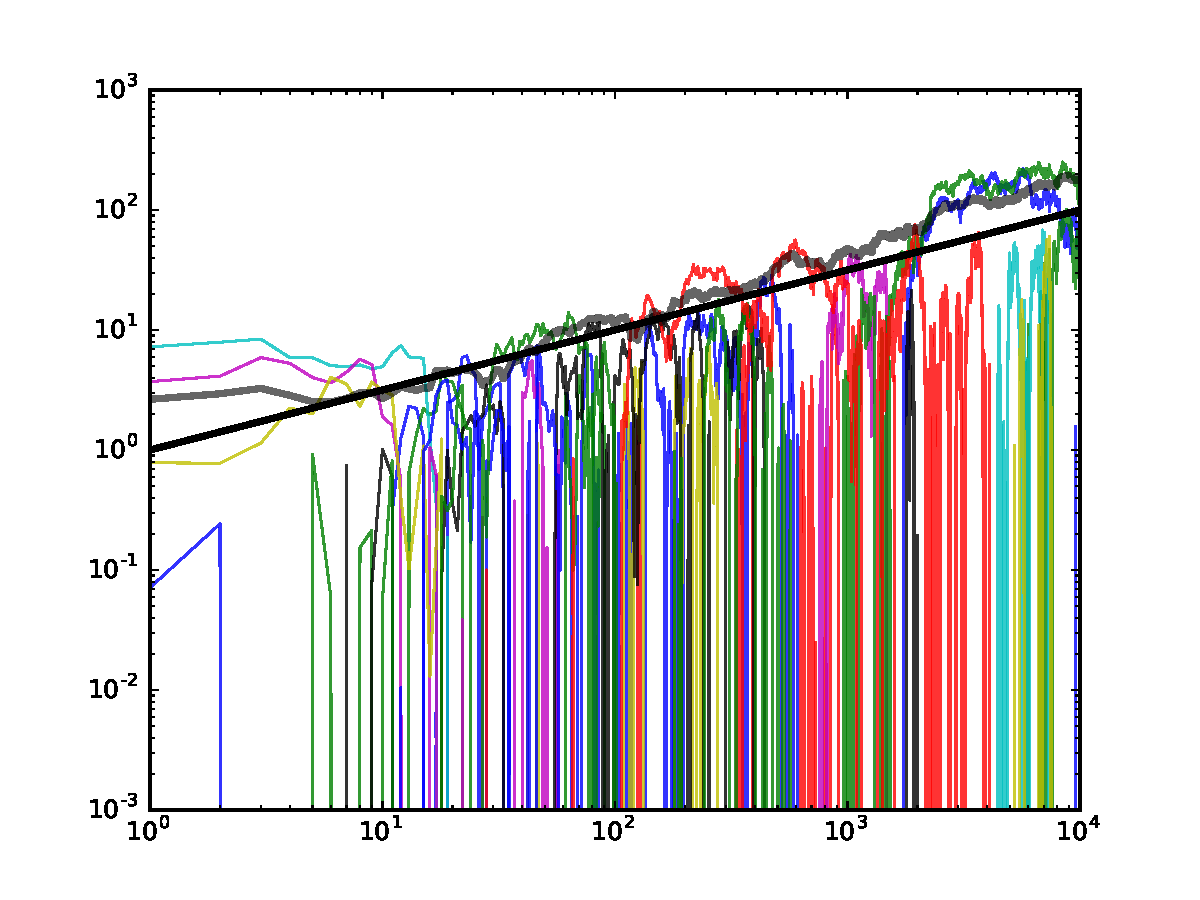
\includegraphics[width=0.5\textwidth]{figures/1_5__1__log.pdf}
    \label{fig:randomwalk_q-gaussian_1.5_log}
  \end{figure}

  \pagebreak

  \begin{figure}[htb]
    \caption{Distribuição q-Gaussiana ($q = 2.0$)}
    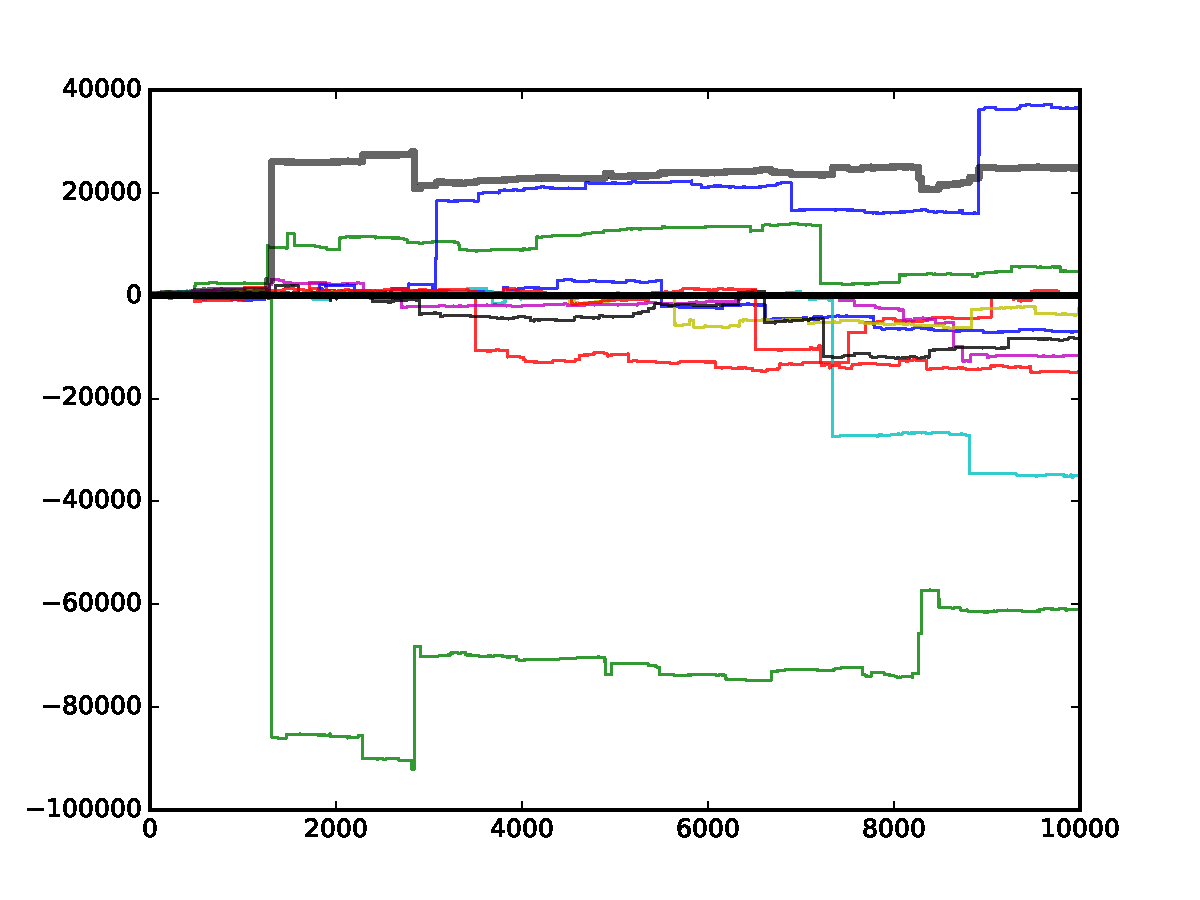
\includegraphics[width=0.5\textwidth]{figures/2_0__0.pdf}
    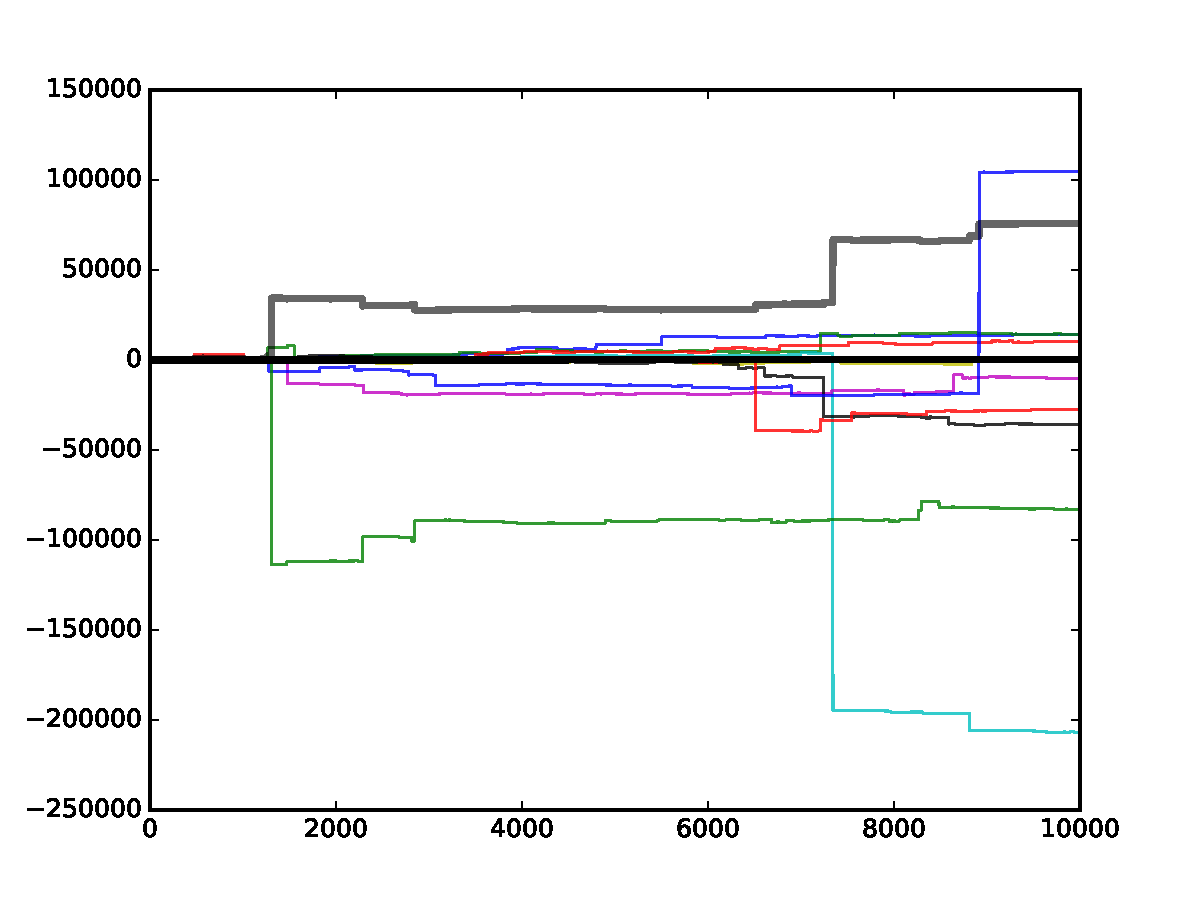
\includegraphics[width=0.5\textwidth]{figures/2_0__1.pdf}
    \label{fig:randomwalk_q-gaussian_2.0}
  \end{figure}

  \begin{figure}[htb]
    \caption{Distribuição q-Gaussiana ($q = 2.0$, escala log)}
    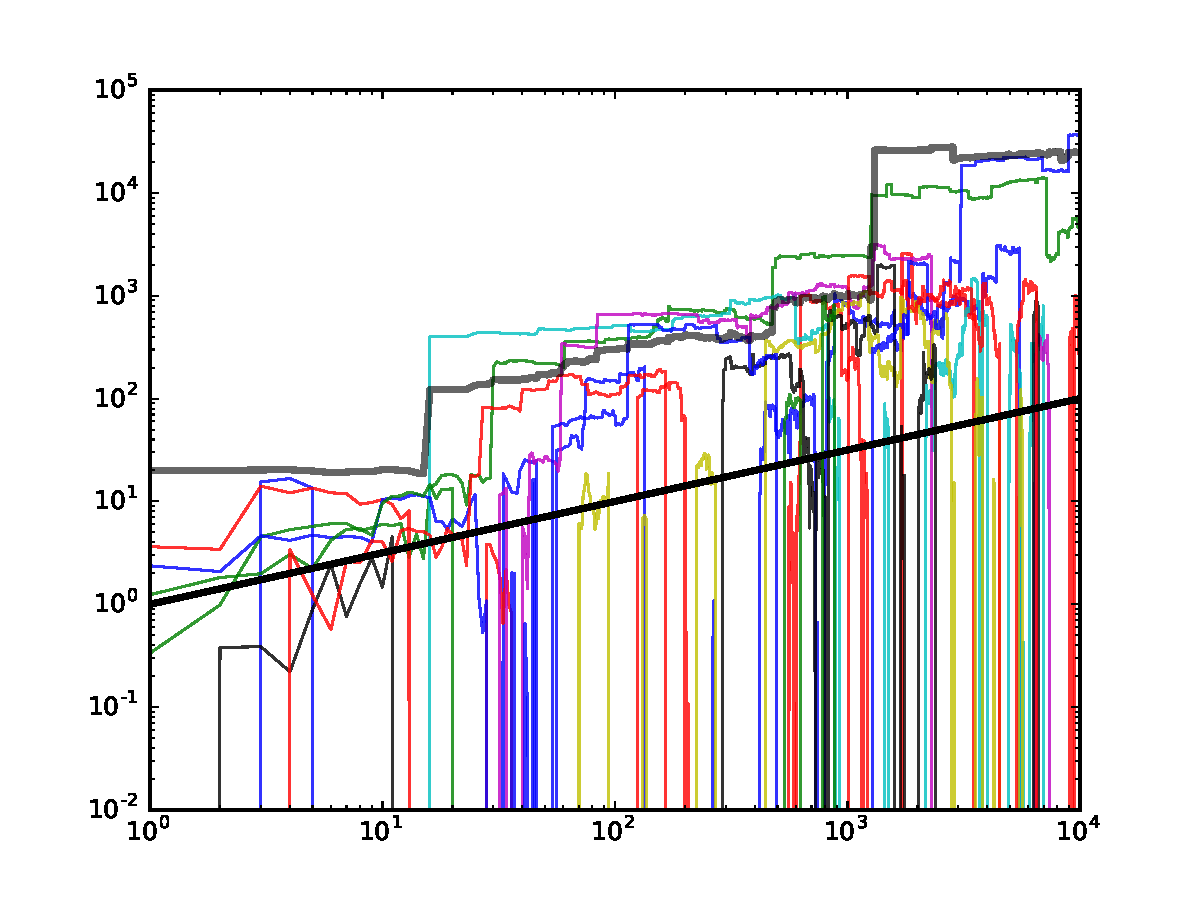
\includegraphics[width=0.5\textwidth]{figures/2_0__0__log.pdf}
    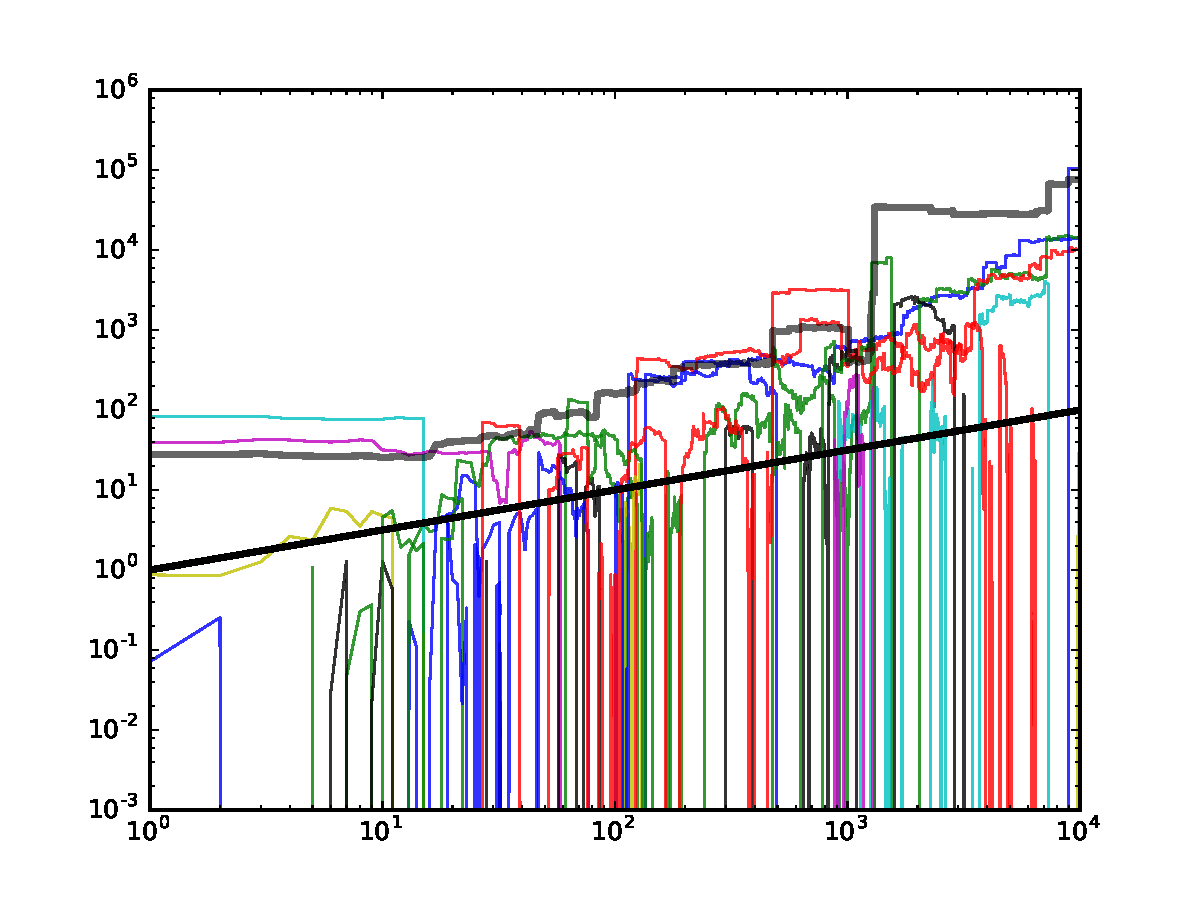
\includegraphics[width=0.5\textwidth]{figures/2_0__1__log.pdf}
    \label{fig:randomwalk_q-gaussian_2.0_log}
  \end{figure}

  \pagebreak

  \begin{figure}[htb]
    \caption{Distribuição q-Gaussiana ($q = 2.5$)}
    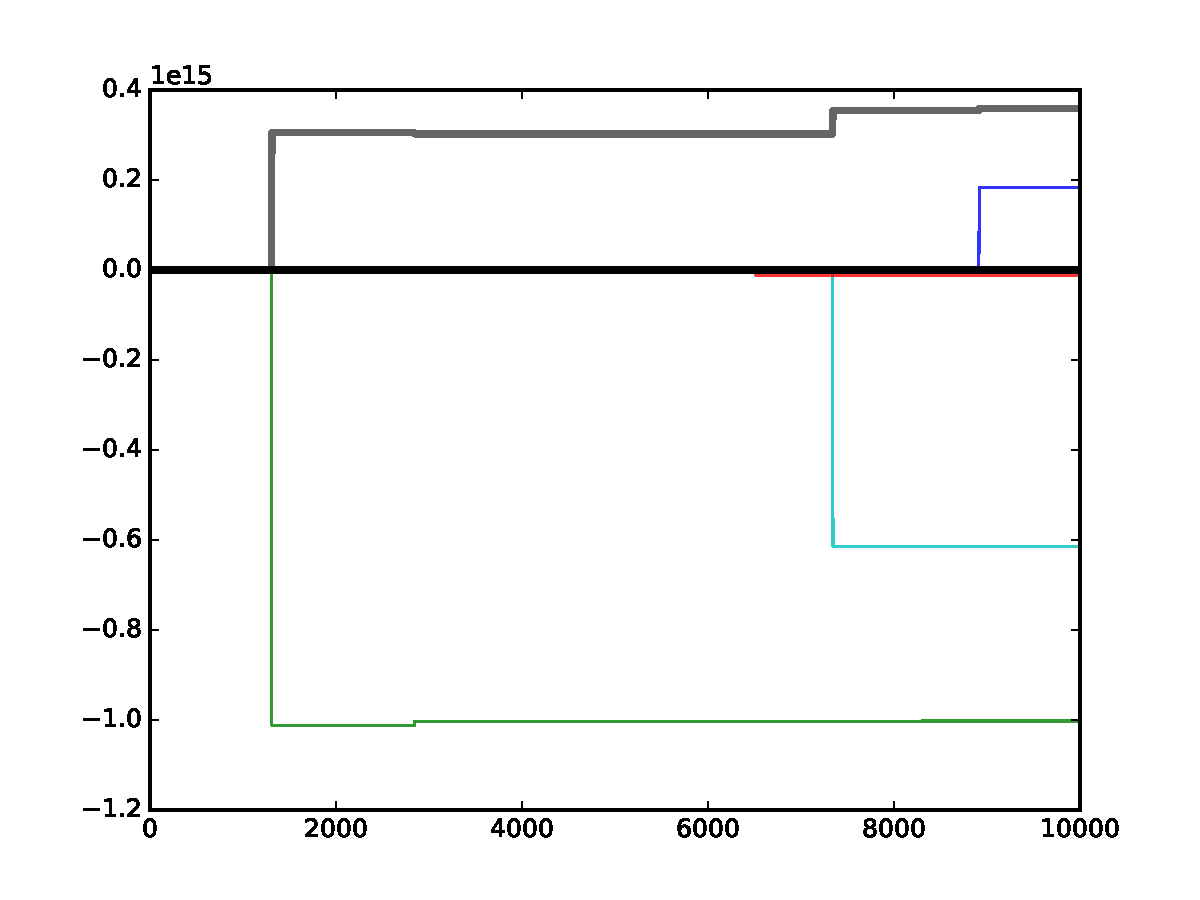
\includegraphics[width=0.5\textwidth]{figures/2_5__0.pdf}
    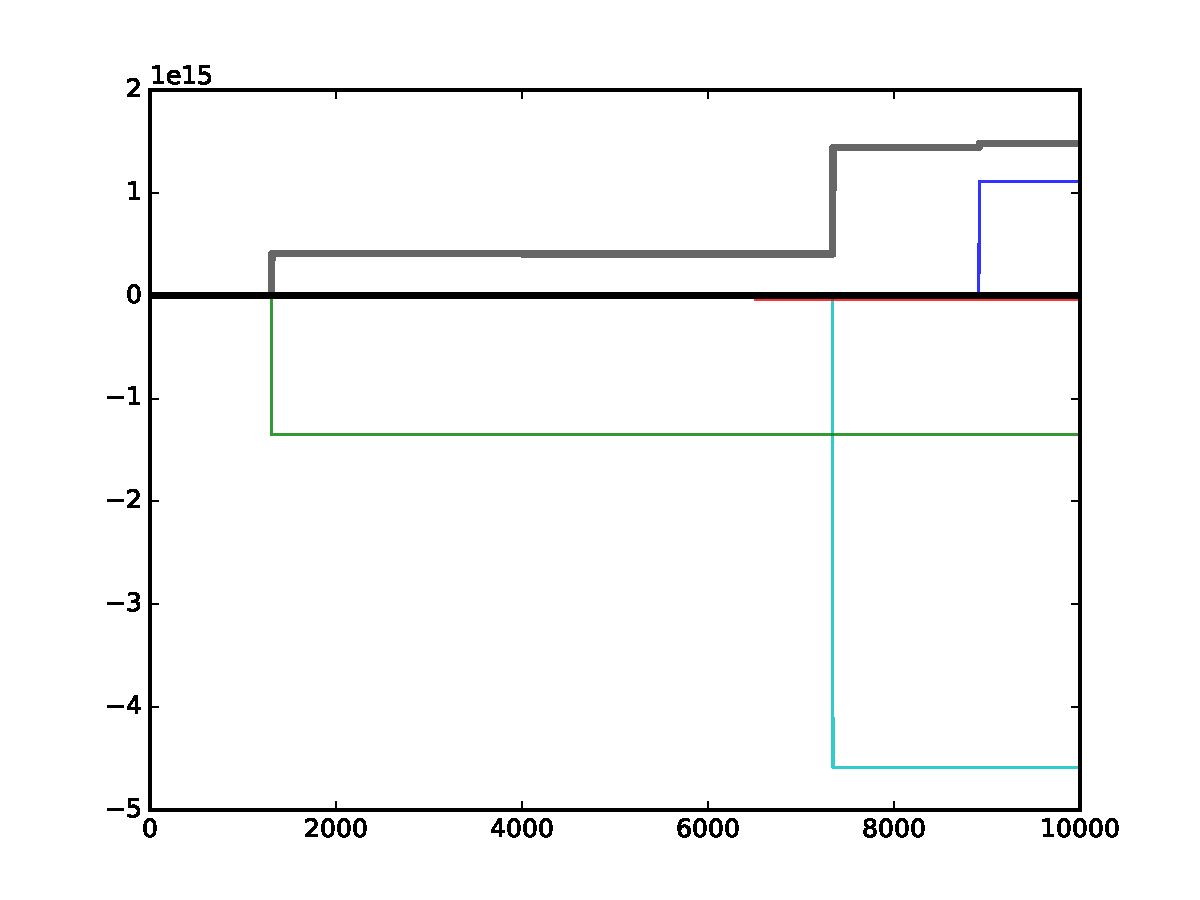
\includegraphics[width=0.5\textwidth]{figures/2_5__1.pdf}
    \label{fig:randomwalk_q-gaussian_2.5}
  \end{figure}

  \begin{figure}[htb]
    \caption{Distribuição q-Gaussiana ($q = 2.5$, escala log)}
    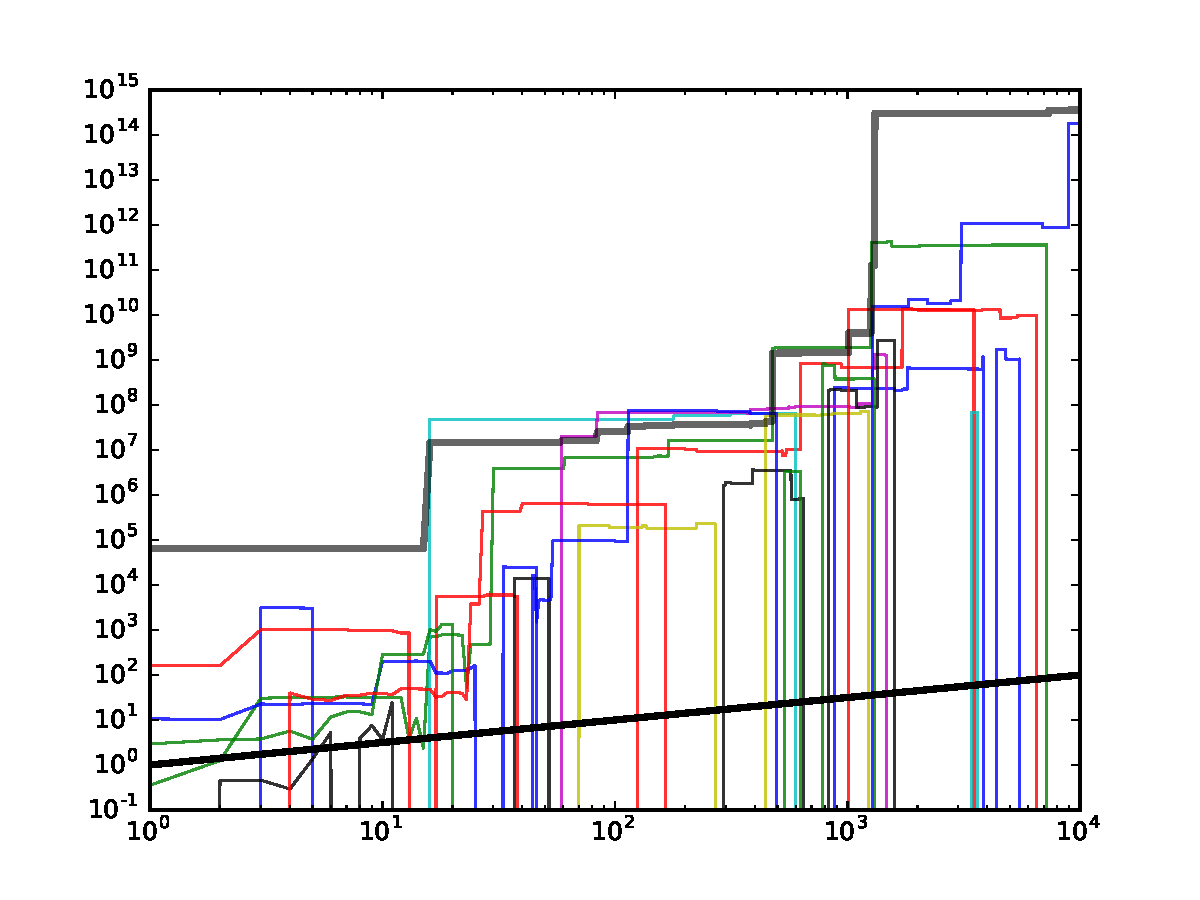
\includegraphics[width=0.5\textwidth]{figures/2_5__0__log.pdf}
    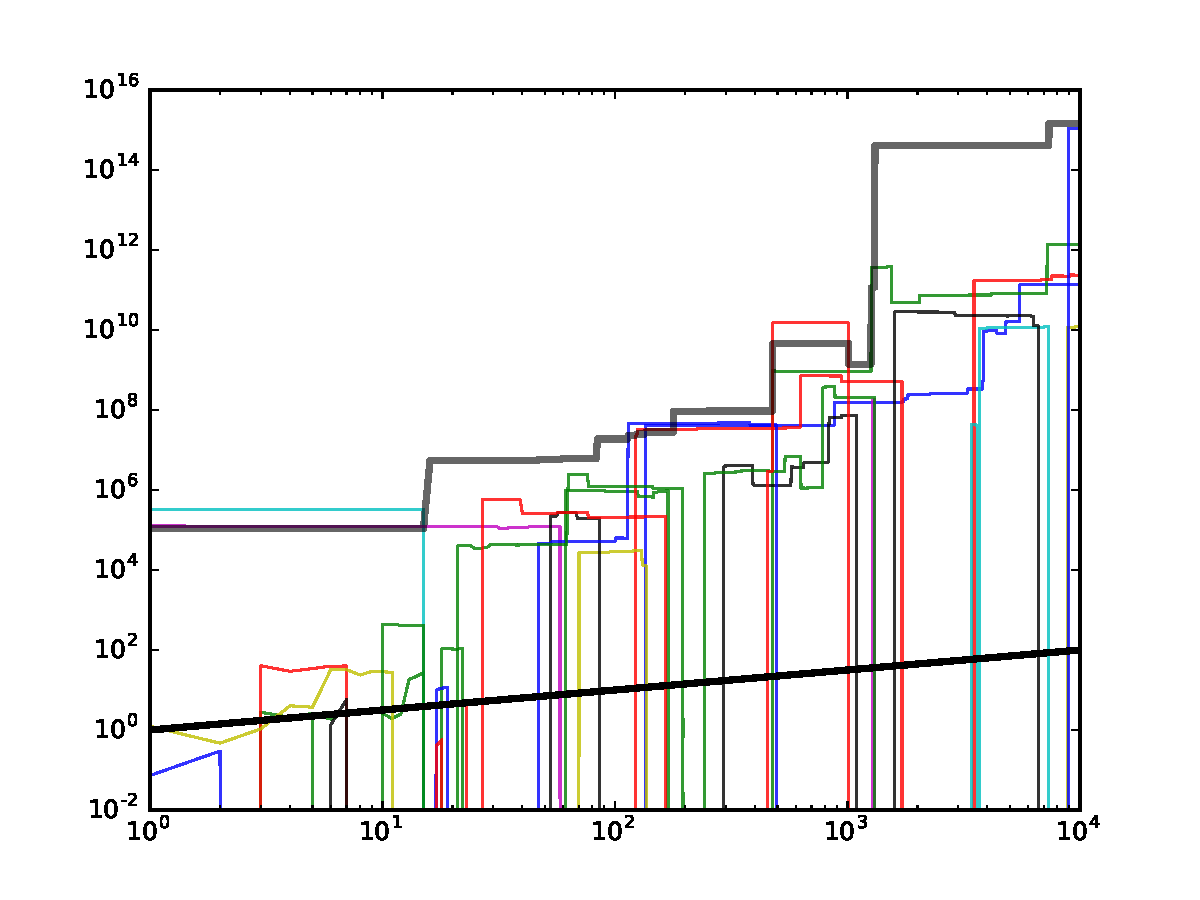
\includegraphics[width=0.5\textwidth]{figures/2_5__1__log.pdf}
    \label{fig:randomwalk_q-gaussian_2.5_log}
  \end{figure}

  \pagebreak

  \section{Referências}
    \vspace{-10mm}
    \bibliographystyle{abbrv}
    \bibliography{refbase.bib}

  % 
\section{Anexos}


\end{document}
